\section{Компьютерная имитация макроэкономических моделей } 

При виконанні дипломної роботи була розроблена програма, що емулює бімитричну гру на часових шкалах та доводить емпірично приведенні в роботі результати. 

Розробка програмного продукту проводилась мовою Python 3.4.
Програма дозволяє користувачеві задати $r^g$, $r^p$ та відповідні скалярні функції поведінки гравця в означений момент часу. Значеннями даної функції буде ймовірність вибору гравцем стратегії $H$ у даний період часу. Також користувач може задати кількість запусків гри с вхідними даними для підрахунку статистики. В якості інтерфейсу вхідних даних було обрано простий текстовий файл, що за необхідності дозволяє будувати великі послідовності експериментів.

\subsection{Аналіз стійкості стратегій у моделі Барро-Гордона}
Нехай матриця виграшів двух гравців відповідає~\ref{table:sec:ot:real},
$r^g= 7$ (кількість ходів уряду), $r^p= 4$ (кількість ходів громадськості).

\begin{table}[h]
	\centering
	
	\caption{}	
			 Матриця виграшів для моделі Барро-Гордона\\
			\normalsize
			
\begin{tabular}{|l|l|c|c|}
	\hline
	\multicolumn{2}{|l|}{\multirow{2}{*}{}} & \multicolumn{2}{l|}{Громадськість} \\ \cline{3-4} 
	\multicolumn{2}{|l|}{}                  & L                & H                \\ \hline
	\multirow{2}{*}{Уряд}    & L   & 0, 0             & -1,-1            \\ \cline{2-4} 
	& H   & $\frac{1}{2}$,-1             & $-\frac{1}{2}$, 0            \\ \hline
\end{tabular}

	\label{table:sec:ot:real1}
\end{table}

Перевіримо виповнення умови теореми~\ref{eq:sec:tech:theoremSystem} для матриці виграшів~\ref{table:sec:ot:real1}. 
$$
r^g> \bar{r^g}(R) = \left\{ 
\begin{aligned} 
&2r^p= 2r^p, &&\text{якщо } R=0
\\
&2(1+R)r^p= 2(1+R)r^p, &&\text{якщо } 	R\in\left(0; \frac{1}{2}\right)
\\
&2Rr^p= 2Rr^p, &&\text{якщо } 	R\in\left( \frac{1}{2};1\right)
\end{aligned}
\right.		
$$
$$
r^g> \bar{r^g}(R) = 0$$
$$
4 > 0
$$
Відповідно $\frac{r^g}{r^p} \in \left(\frac{3}{2};2\right)$ обрані вірно та усі досконалі рівноваги по під-іграм повинні бути досконалими рівновагами по под-іграм Рамсея.
 
Проаналізуємо випадок, коли уряд є більш схильним ввести високий рівень інфляції, а громадськість припускаючи, що уряд піде на такий крок з високим рівнем ймовірності, підіймає заробітні плати.

Задамо розподіл ймовірностей обрання стратегії $H$ для кожного з двох гравців:
 \begin{gather*}
 	q^g = \left[ 0.5; 0.9; 0.7; 0.5; 0.9; 0.73; 0.8 \right], \\
 	q^p = \left[ 0.8; 0.9; 0.8; 1 \right].
 \end{gather*}
За допомогою програми проведемо емуляцію 100 ігор з такими початковими даними.

\begin{figure}[h]
	\centering
		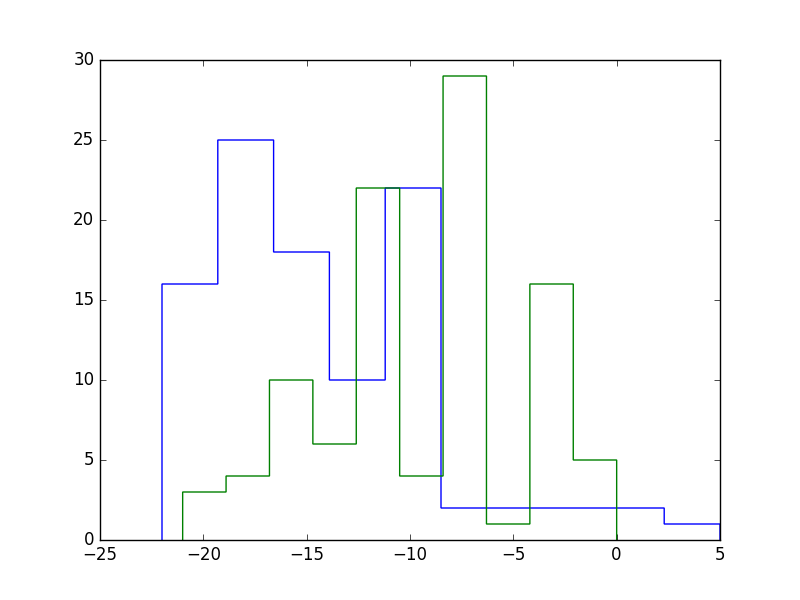
\includegraphics[width=0.5\linewidth]{Public1.png}
			
	\caption{Гістограма виграшів, синій -- уряд, зелений -- громадськість}
	\label{fig:stat1}
\end{figure}

\begin{table}[h]
	\centering
	\caption{}
	 Статистичні показники для 100 ігр\\
			\normalsize
			
	\begin{tabular}{|l|c|c|}
		\hline
		& Уряд & Громадськість \\ \hline
		Середнє                                                           & -14.26        & -9.46          \\ \hline
		\begin{tabular}[c]{@{}l@{}}Стандартне \\ відхилення\end{tabular} & 5.34          & 4.66           \\ \hline
		Асиметріяя                                                        & 1.1           & -0.041         \\ \hline
		Эксцес                                                           & 1.37          & -0.37          \\ \hline
	\end{tabular}
\end{table}

Згідно з отиманими результатами легко бачити, що подібний набір стратегій є невигідним обом сторонам, до того ж уряду через більш "м'який" підхід "більш невигядно".

Розглянемо випадок, коли уряд на останньому кроці може відступити від оптимальної для обох гравців стратегії $ (L, L) $.

Задамо розподіл ймовірностей вибору даної стратегії для кожного з двох гравців:
 \begin{gather*}
 	q^g = \left[ 0; 0; 0; 0; 0; 0; 0.3 \right], \\
 	q^p = \left[ 0; 0; 0; 0 \right].
 \end{gather*}


\begin{figure}[h]
	

		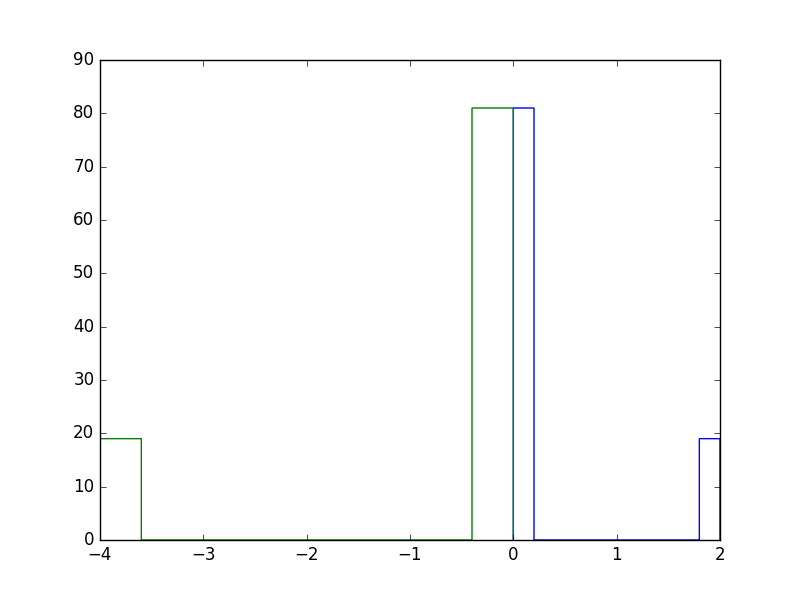
\includegraphics[width=0.5\linewidth]{Public.png}
	\centering	
	\caption{Гістограма виграшів, синій - уряд, зелений - громадськість}
	\label{fig:stat}
\end{figure}

\begin{table}[h]
	\centering
		\caption{}
	Статистичні показники для 100 ігор\\
		\normalsize
	\begin{tabular}{|l|l|l|}
		\hline
		& Уряд & \multicolumn{1}{c|}{Громадськість} \\ \hline
		Середнє                                                           & 0.39        & -0.78                         \\ \hline
		\begin{tabular}[c]{@{}l@{}}Стандартне \\ відхилення\end{tabular} & 0.78         & 1.56                          \\ \hline
		Асиметрія                                                        & 1.6          & -1.11                          \\ \hline
		Эксцес                                                           & 0.58        & 0.58                        \\ \hline
	\end{tabular}
\end{table}

Дана стратегія є виграшною для уряду, якщо громадськість не очікує подібного кроку під кінець дії терміну уряду.

Розглянемо випадок, коли громадськість довіряє уряду і майже впевнено, що воно не може підняти рівень інфляції до закінчення терміну свого правління.

Задамо розподіл ймовірностей вибору даної стратегії для кожного з двох гравців:
 \begin{gather*}
 	q^g = \left[ 0; 0; 0; 0; 0; 0; 0.3 \right], \\
 	q^p = \left[ 0; 0; 0; 0.15 \right].
 \end{gather*}
	\begin{figure}[h]
		
\centering
				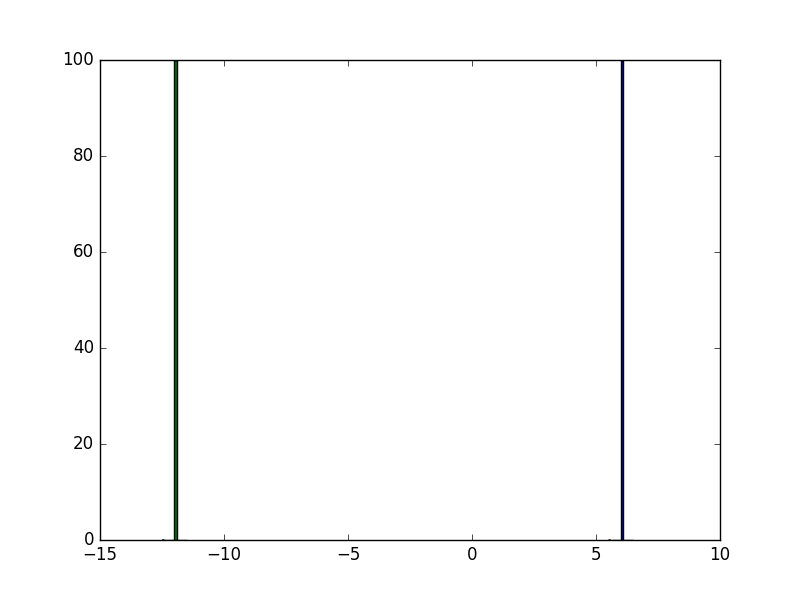
\includegraphics[width=0.5\linewidth]{Public2.png}
		
		\caption{Гістограма виграшів, синій - уряд, зелений - громадськість}
		\label{fig:stat2}
	\end{figure}
	\begin{table}[h]
		\centering
			\caption{}
		 Статистичні показники для 100 ігор\\
			\normalsize
 \begin{tabular}{|l|c|c|}
 	\hline
 	& Уряд & Громадськість \\ \hline
 	Середнє                                                           & -0.9          & -2.18          \\ \hline
 	\begin{tabular}[c]{@{}l@{}}Стандартне \\ відхилення\end{tabular} & 3          & 2.58           \\ \hline
 	Асиметрія                                                        & -1.16           & -0.68          \\ \hline
 	Эксцес                                                           & -0.06          & -0.95           \\ \hline
 \end{tabular}
	\end{table}
	
Легко бачити, що дана стратегія однозначно погіршує позицію уряду, але так само не вигідна громадськості.

Розглянемо випадок, коли громадськість не довіряє уряду і майже впевнено, що воно підвищить рівень інфляції до закінчення терміну свого правління.
  Задамо розподіл ймовірностей вибору даної стратегії для кожного з двох гравців:
 \begin{gather*}
 	q^g = \left[ 0; 0; 0; 0; 0; 0; 0.3 \right], \\
 	q^p = \left[ 0; 0; 0; 0.8 \right].
 \end{gather*}
 	\begin{figure}[h]
 		\centering
 			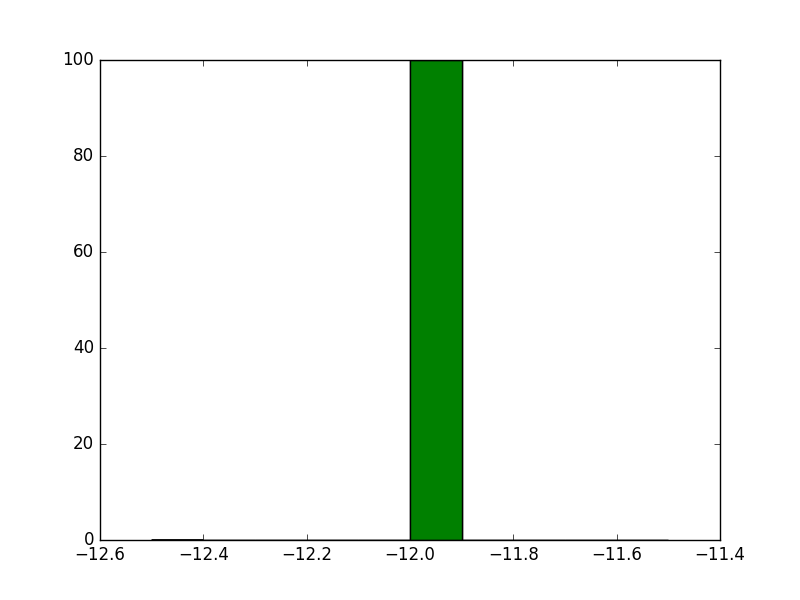
\includegraphics[width=0.5\linewidth]{Public3.png}
 		\caption{Гістограма виграшів, синій - уряд, зелений - громадськість}
 		\label{fig:stat3}
 	\end{figure}
 	
 	\begin{table}[h]
 		\centering	\caption{}
 		 Статистичні показники для 100 ігор\\
 		\normalsize
 	 \begin{tabular}{|l|c|c|}
 	 	\hline
 	 	& Уряд & Громадськість \\ \hline
 	 	Середнє                                                           & -4.8          & -4.62          \\ \hline
 	 	\begin{tabular}[c]{@{}l@{}} Стандартне \\ відхидення\end{tabular} & 2.99          & 2.65           \\ \hline
 	 	Асиметрія                                                        & 1.18           & 0.54          \\ \hline
 	 	Эксцес                                                           & -0.12          & -1.15           \\ \hline
 	 \end{tabular}
 	\end{table}	
Дана стратегія є рівносильно невигідна для обох гравців.
 \newpage
У зв'язку з отриманими результатами можна зробити висновок, що якщо уряд
має більше кроків на часових шкалах, то йому має сенс відхилиться від
оптимальної по Парето стратегії $ (L, L) $ і підвищити рівень інфляції під кінець
терміну свого правління, так як навіть якщо громадськість чекатиме такого
ходу, то з метою мінімізувати свої втрати не підвищуватиме індексування
заробітної плати заздалегідь. Цілком природньо якщо уряд захоче заручитися
підтримкою громадськості на наступних виборах, то такий крок з його боку буде
схлжий на "політичне самогубство".

\subsection{Аналіз стійкості стратегій в моделі профспілка~-- монополіст}
Покладемо матрицю виграшів відповідно до~\ref{table:firm} наступним чином:
\newpage
\begin{table}[h]
	
	\centering
	\caption{}
	Матриця вииграшів наступна~(\ref{table:firm})\\
	\normalsize
\begin{tabular}{|l|l|c|c|}
	\hline
	\multicolumn{2}{|l|}{\multirow{2}{*}{}} & \multicolumn{2}{l|}{Профсоюз} \\ \cline{3-4} 
	\multicolumn{2}{|l|}{}                  & L            & H              \\ \hline
	\multirow{2}{*}{Фірма}        & L       & 3, 1         & 2, 3.9         \\ \cline{2-4} 
	& H       & 7, 4         & -3, 7          \\ \hline
\end{tabular}
	\label{table:mono:ex}
\end{table}
Для знахождения равноваги по Нэшу підрахуємо наступне: \\
Фірма
	$$ L:  3\alpha + 2(1-\alpha)=\alpha + 2$$
	$$ H: 7\alpha - 3(1-\alpha)=10\alpha - 3$$
	$$10\alpha - 3 = \alpha+2 $$
	$$\alpha = \frac{5}{9} $$
Профсоюз	
	 $$L: \beta + 4(1-\beta)=-3\beta + 4$$
	 $$H: 3.9\beta + 7(1-\beta)=-3.1\beta +7$$
	$$0.1\beta  = 3 $$
	$$\beta = 30 $$
Отже рівновагою Неша буде стратегія $L,H$.

У кожному стовпці матриці фірми знайдемо максимальний елемент.
Потім в кожному рядку матриці профспілки виберемо найбільший елемент.
Платіжна матриця фірми:
\begin{table}[h]
	\centering
	\begin{tabular}{|l|l|}
		\hline
		3, 1 & \textbf{2, 3.9}  \\ \hline
		\textbf{7}, 4 & -3, \textbf{7} \\ \hline
	\end{tabular}
\end{table}\\
Оптимальною по Парето буде стратегія $ (H, L) $. Далі вважаємо $ r^f = 4 $ (кількість кроків фірми за одну гру), $ R^p = 3 $ (кількість кроків профспілки). 

 Розглянемо випадок, коли обидва гравці намагаються слідувати рівноважній стратегії
  Неша. Задамо розподіл ймовірностей вибору першої стратегії для
  кожного з двох гравців:
 \begin{gather*}
 	q^f = \left[ 0.9; 0.9; 0.9; 0.9 \right], \\
 	q^p = \left[ 0.1; 0.1; 0.1 \right].
 \end{gather*}

 	\begin{figure}[h]
 		\centering
 		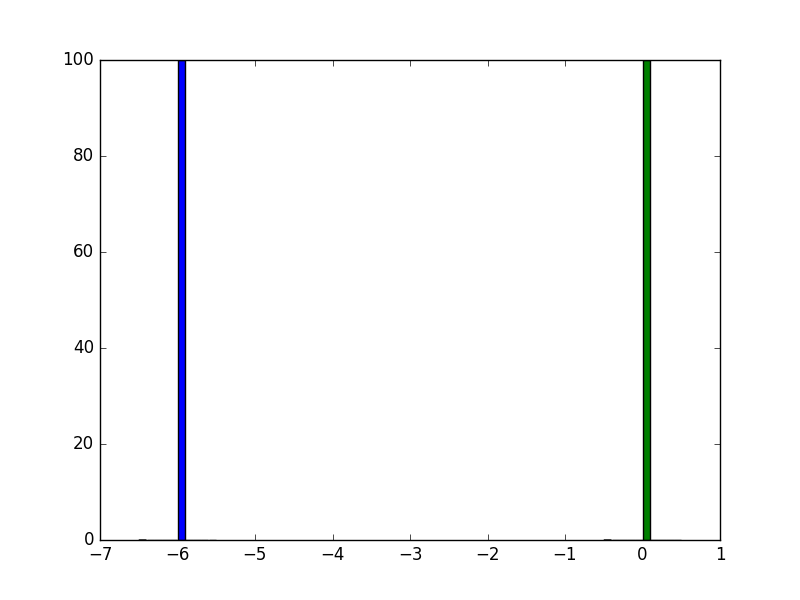
\includegraphics[width=0.5\linewidth]{Public4.png}
 		\caption{Гістограма виграшів, синій - фірма, зелений - профспілка}
 		\label{fig:stat4}
 	\end{figure}
 	
 	\begin{table}[h]
 		\centering
 			\caption{}
 			Статистичні показники для 100 ігор\\
 			\normalsize
 		 \begin{tabular}{|l|c|c|}
 		 	\hline
 		 	& Фірма & Профсоюз\\ \hline
 		 	Середнє                                                           & 69.02          & 47.84          \\ \hline
 		 	\begin{tabular}[c]{@{}l@{}}Стандартне \\ відхилення\end{tabular} & 18.1          & 8.19           \\ \hline
 		 	Асиметрія                                                        & -1.04           & 0.017          \\ \hline
 		 	Эксцес                                                           & 0.25         & 0.69           \\ \hline
 		 \end{tabular}
 	\end{table}
 	
\newpage
 Розглянемо випадок, коли профспілка намагається збільшувати зарплату на своєму
  останньому кроці, а фірма для виходу з нерентабельного положення скорочує
  кількість співробітників. Задамо розподіл ймовірностей вибору даної
  стратегії для кожного з двох гравців:
 \begin{gather*}
 	q^f = \left[ 0.9; 0.9; 0.9; 0.1 \right], \\
 	q^p = \left[ 0.1; 0.1; 0.9 \right].
 \end{gather*}
 
\begin{figure}[h]
 		\centering
 		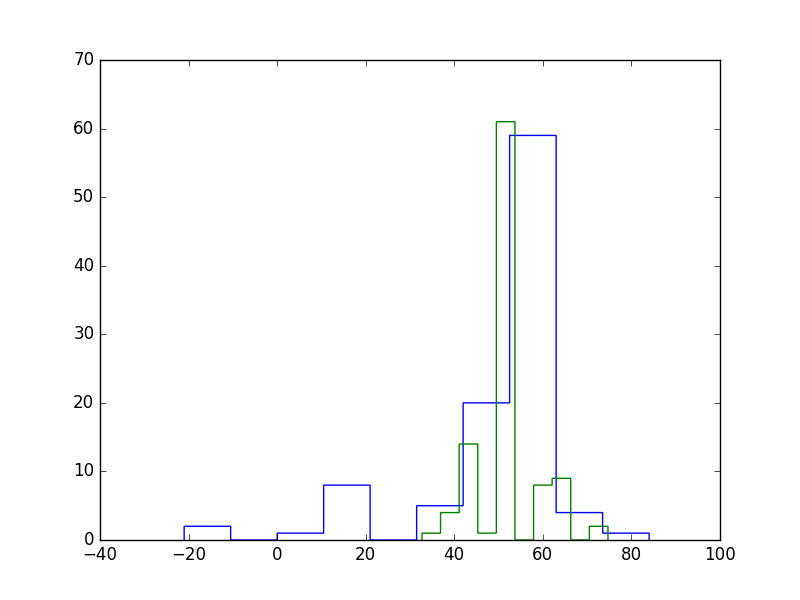
\includegraphics[width=0.5\linewidth]{Public5.png}
 		\caption{Гістограма виграшів, синій - фірма, зелений - профспілка}
 		\label{fig:stat5}
 	\end{figure}
 	
 	\begin{table}[h]
 		\centering
 			\caption{}
 			Статистичні показники для 100 ігор\\
 			\normalsize
 		 \begin{tabular}{|l|c|c|}
 		 	\hline
 		 	& Фірма & Профсоюз\\ \hline
 		 	Середнє                                                           & 50.48      &  51.1                        \\ \hline
 		\begin{tabular}[c]{@{}l@{}}Стандартне \\ відхилення\end{tabular} & 17.18        &  7.17                          \\ \hline
 		Асиметрія                                                        & -2.02          &0.57                          \\ \hline
 		Эксцес                                                           & 5.21        & 1.44                        \\ \hline
 	\end{tabular}
 \end{table}
Така стратегія незначно поліпшить позиції профспілки, але помітно похитне позицію фірми.
\newpage
  Розглянемо випадок, коли профспілка збільшить зарплату вдруге і повернеться до
  оптимальної стратегії на третій період. Задамо розподіл ймовірностей
  вибору даної стратегії для кожного з двох гравців:
 \begin{gather*}
 	q^f = \left[ 0.9; 0.9; 0.1; 0.9 \right], \\
 	q^p = \left[ 0.1; 0.9; 0.1 \right].
 \end{gather*}
 \begin{figure}[h]
 	\centering
 	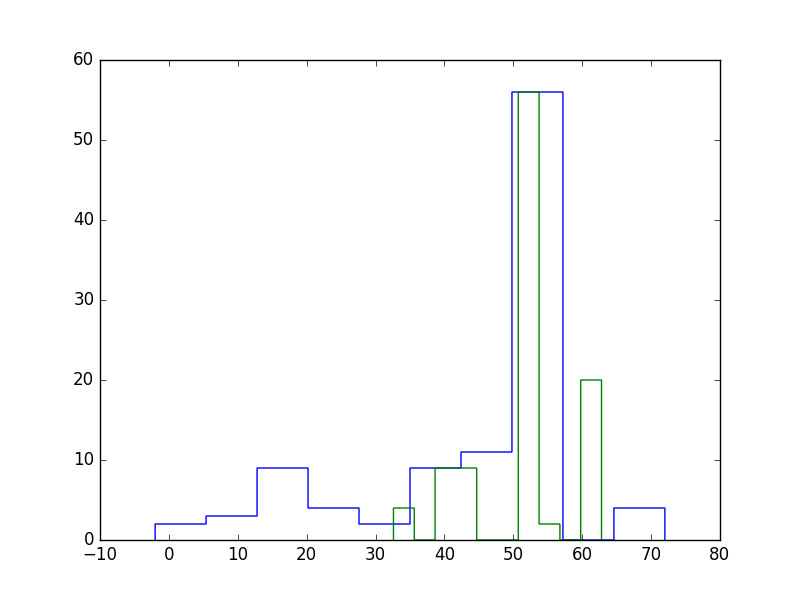
\includegraphics[width=0.5\linewidth]{Public6.png}
 	\caption{Гістограма виграшів, синій - фірма, зелений - профспілка}
 	\label{fig:stat6}
 \end{figure}
 
 \begin{table}[h]
 	\centering
 		\caption{}
 		Статистичні показники для 100 ігор\\
 		\normalsize
  \begin{tabular}{|l|c|c|}
  	\hline
  	& Фірма & Профсоюз\\ \hline
  		Середнє                                                           & 43.06      &  50.64                        \\ \hline
 		\begin{tabular}[c]{@{}l@{}}Стандартне \\ відхилення\end{tabular} & 14.47        &  7.38                          \\ \hline
 		Асиметрія                                                        & -1.06          &-0.29                          \\ \hline
 		Эксцес                                                           & 1.30       &0.09                        \\ \hline
 	\end{tabular}
 \end{table}
 
Знову таки разова акція підняття зарплат дає профспілці незначний виграш, але фірма при цьому програє відносно набагато більше, ніж виграє профспілка.
\newpage
  Розглянемо випадок, коли профспілка піднімає на другому своєму ході зарплату, але
  не опускає його аж до кінця гри. Задамо розподіл ймовірностей
  вибору цієї стратегії для кожного з двох гравців:
  \begin{gather*}
  	q^f = \left[ 0.9; 0.9; 0.1; 0.2 \right], \\
  	q^p = \left[ 0.1; 0.9; 0.8 \right].
  \end{gather*}
  \begin{figure}[h]
  	\centering
  	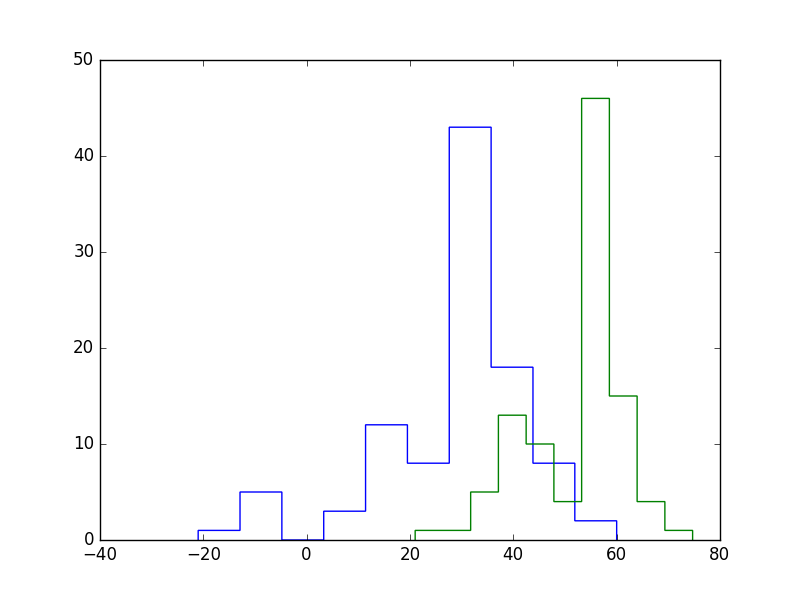
\includegraphics[width=0.5\linewidth]{Public7.png}
  	\caption{Гістограма виграшів, синій - фірма, зелений - профспілка}
  	\label{fig:stat7}
  \end{figure}
  
  \begin{table}[h]
  	\centering
  		\caption{}
  	 Статистичні показники для 100 ігор\\
  		\normalsize
   \begin{tabular}{|l|c|c|}
   	\hline
   	& Фірма & Профсоюз\\ \hline
   		Середнє                                                           & 30.37     &  51.37                        \\ \hline
  		\begin{tabular}[c]{@{}l@{}}Стандартне \\ відхилення\end{tabular} & 13.64        &  8.99                          \\ \hline
  		Асиметрія                                                        & -1.36         &-0.53                          \\ \hline
  		Эксцес                                                           & 2.74       & 0.8                        \\ \hline
  	\end{tabular}
  \end{table}

  \newpage
Фірма знову втрачає в відносних грошах, в той час як профспілка тільки
незначно покращує своє становище. Розумно з точки зору фірми зробити
пропозицію профспілці не змінювати рівень зарплат з оптимального, а натомість
відплачувати різними видами бонусів. Тоді функція корисності зміниться для обох
гравців на рівну величину. Фірмі варто підібрати цю величину бонусів так,
щоб залишок між її оптимальним виграшем після вирахування бонусів був чимось
середнім між власними виграшами, коли профспілка встановлює високий
рівень зарплат і низький.
